\documentclass[10pt]{article}
\usepackage[a4paper,margin=14mm,top=12mm,bottom=12mm]{geometry}
\usepackage{fontspec}
\setmainfont{TeX Gyre Heros}
\usepackage{graphicx,tikz,array,tabularx,enumitem,multicol,booktabs}
\usepackage[most]{tcolorbox}
\usepackage{xcolor}
\usepackage{amssymb}
\pagestyle{empty}
\setlength{\parindent}{0pt}
\setlength{\parskip}{3pt}
\setlist{nosep,leftmargin=*}
\frenchspacing
\newcommand{\sh}{$\sharp$}
\newcommand{\fl}{$\flat$}

% ---------- headings
\newcommand{\sect}[1]{\par\vspace{5pt}{\large\bfseries #1}\par\vspace{2pt}}

% ---------- drill header
\newcommand{\drill}[6]{%
\noindent
\begin{tikzpicture}[baseline=(b.base)]
\node[fill=black,minimum width=15mm,minimum height=15mm,text=white,inner sep=0,rounded corners=1pt] (b) {};
\node[text=white,font=\sffamily\bfseries\tiny] at ([yshift=-2.3mm]b.north) {DRILL};
\node[text=white,font=\sffamily\bfseries\fontsize{24}{24}\selectfont] at ([yshift=-1.5mm]b.center) {#1};
\end{tikzpicture}\hspace{4mm}%
\begin{minipage}[b]{0.86\textwidth}
{\fontsize{20}{22}\selectfont\bfseries #2}\\[1pt]
{\itshape #3}\\[1pt]
{\small\textbf{Needs:} #4\quad \textbf{Skills:} #5\quad \textbf{Gate:} #6}
\end{minipage}\par\vspace{2pt}
\noindent\rule{\textwidth}{0.8pt}\par\vspace{3pt}}

\newtcolorbox{why}{enhanced,colback=white,colframe=black,boxrule=0.5pt,arc=2mm,
  colbacktitle=black!12,coltitle=black,fonttitle=\small\bfseries,title=Why this matters,
  left=2mm,right=2mm,top=1.5mm,bottom=1.5mm,before skip=2pt,after skip=4pt}
\newtcolorbox{sidebox}[1]{enhanced,colback=white,colframe=black,boxrule=0.5pt,arc=2mm,
  colbacktitle=black!12,coltitle=black,fonttitle=\small\bfseries,title=#1,
  left=2mm,right=2mm,top=1mm,bottom=1mm,fontupper=\small,equal height group=bottom\thepage}
\newtcolorbox{greybox}{enhanced,colback=black!6,colframe=black!6,arc=2mm,left=2mm,right=2mm,top=1mm,bottom=1mm,fontupper=\small}

% ---------- 5 minutes
\newcommand{\tm}[1]{\fbox{\scriptsize\bfseries\strut #1}}
\newenvironment{fivemin}{\sect{The 5 minutes}\small\renewcommand{\arraystretch}{1.25}\tabularx{\textwidth}{@{}p{17mm}X@{}}}{\endtabularx}

% ---------- ladder
\newcommand{\cb}{\framebox(7,7){}}
\newenvironment{ladder}{\begin{tcolorbox}[enhanced,colback=white,colframe=black,boxrule=0.8pt,arc=2mm,
  colbacktitle=black!12,coltitle=black,fonttitle=\small\bfseries,
  title={Level ladder --- stay on a level for days or weeks; tick it when you play it clean 3 times in a row},
  left=0mm,right=0mm,top=0.5mm,bottom=0.5mm,before skip=4pt,after skip=4pt]\small
  \renewcommand{\arraystretch}{1.12}\begin{tabular}{@{\hspace{1mm}}c@{\hspace{1.5mm}}l@{\hspace{1.5mm}}p{0.745\linewidth} r@{\hspace{2mm}}p{13mm}@{}}}
  {\end{tabular}\end{tcolorbox}}
\newcommand{\lv}[3]{\cb & \textbf{#1} & #2 & \footnotesize #3 & \rule[-1pt]{13mm}{0.4pt}\\}

\newcommand{\bottom}[2]{\par\vspace{2pt}\noindent
\begin{tcbraster}[raster columns=2,raster equal height,raster column skip=3mm,
  enhanced,colback=white,colframe=black,boxrule=0.5pt,arc=2mm,colbacktitle=black!12,coltitle=black,
  fonttitle=\small\bfseries,left=2mm,right=2mm,top=1mm,bottom=1mm,fontupper=\small]
\begin{tcolorbox}[title=Make it harder]#1\end{tcolorbox}
\begin{tcolorbox}[title=In the recording]#2\end{tcolorbox}
\end{tcbraster}}

\newcommand{\blank}[1][25mm]{\rule[-1pt]{#1}{0.4pt}}

% ---------- rhythm grid
\newcommand{\hit}{\tikz[baseline=-0.6ex]\fill (0,0) circle (2.1pt);}
\newcommand{\hold}{\tikz[baseline=-0.6ex]\draw[line width=0.9pt] (-1.8mm,0) -- (1.8mm,0);}
\newcommand{\no}{\tikz[baseline=-0.6ex]\fill[black!50] (0,0) circle (0.8pt);}

\newcommand{\score}[2][\textwidth]{\par\noindent\includegraphics[width=#1]{ly/#2.cropped.pdf}\par}
\newcommand{\kb}[1]{\input{kbd/#1.tex}}

\begin{document}

%===================================================== COVER
{\fontsize{26}{28}\selectfont\bfseries The Loneliest Girl: Five-Minute Drills}\par\vspace{2pt}
{\large Nine drills for one song, from locking to the tempo to playing the melody over your own left hand}\par
\vspace{2pt}\noindent\rule{\textwidth}{0.8pt}\par\vspace{2pt}

\begin{minipage}[t]{0.485\textwidth}
\sect{What this set is for}
One target: play \textbf{The Loneliest Girl} (Carole \& Tuesday) at the keyboard with both hands, at the record's tempo, with the form in your head.

On the way you pick up the pop-piano toolkit the song is built from: chord shapes that barely move, a left hand that keeps time, the push, broken chords, and finding a melody by ear.

The melody notes are not written out here. Learn them from licensed sheet music or a tutorial. Drill 9 gets your ear and right hand ready so that goes quickly.

\sect{The song at a glance}
\small
\renewcommand{\arraystretch}{1.15}
\begin{tabularx}{\linewidth}{@{}>{\bfseries}l X@{}}
Key & G major (one sharp: F\sh)\\
Tempo & about 112 BPM, 4/4\\
Chords & Em, C, G, Bm, D, Am (six in all)\\
Verse & Em -- C -- G -- Bm \hfill vi--IV--I--iii\\
Pre-chorus & C -- G -- Em -- D, C -- G -- Am -- D\\
Chorus & C -- G -- Em -- D, ends C -- D -- G\\
\end{tabularx}\par
\footnotesize Chord charts online disagree in details. Treat this as the skeleton and check it against the recording; Drill 1 has you count the bars yourself.\normalsize

\sect{The daily routine}
\begin{enumerate}
\item \textbf{Set a 5-minute timer.} Stop when it rings, even if it's going well.
\item \textbf{One front drill}: the lowest one whose gate you haven't ticked. With 10 minutes, add one review drill.
\item \textbf{Follow ``The 5 minutes''} on the page. The last minute is always playing, and most days that means playing some of the song.
\end{enumerate}

\sect{Three rules}
\textbf{1. Count out loud.} ``One and two and\dots'' Every time.\par
\textbf{2. Metronome ladder.} Start where you make no mistakes. 3 clean runs: add 5 BPM. Two stumbles in a row: drop 5 BPM.\par
\textbf{3. Slow and clean beats fast and messy.} Your hands learn whatever you repeat, mistakes included.

\sect{When to go back}
If hands together (Drills 6--7) falls apart, the gap is nearly always in the chord shapes (3--4) or the left hand (5). Spend a few days there.
\end{minipage}\hfill
\begin{minipage}[t]{0.485\textwidth}
\sect{How to read the pages}
\begin{greybox}
\begin{minipage}{24mm}\kb{legend}\end{minipage}\hfill
\begin{minipage}{0.64\linewidth}\raggedright
\hit\ black dot = press this key. The label is a \textbf{finger}, a \textbf{scale step}, or R/3/5 (root, third, fifth).\\[1pt]
$\blacktriangle$ triangle = the \textbf{root} or home note.\end{minipage}\par\vspace{3pt}
\textbf{Fingers:} 1 = thumb \dots\ 5 = pinky, both hands.\par
\textbf{Chord symbols:} G = G major, Em = E minor, Bm = B minor.\par
\textbf{Roman numerals} number the chords of the key: I = the chord on step 1 (G), vi = the chord on step 6 (Em). Capitals are major, small letters minor. Drill 2 explains it.\par
\textbf{Rhythm grids} split a 4/4 bar into 8 slots:\par\vspace{2pt}
\centering
\begin{tabular}{*{8}{c}}
\textbf{1}&\textbf{\&}&\textbf{2}&\textbf{\&}&\textbf{3}&\textbf{\&}&\textbf{4}&\textbf{\&}\\
\hit&\hold&\no&\hit&\hold&\no&\hit&\hold\\
\end{tabular}\par\raggedright
\hit\ = play, \hold\ = keep holding, \no\ = nothing new. This one is 3-3-2 (Drill 6).
\end{greybox}

\sect{The map}
\small
\renewcommand{\arraystretch}{1.15}
\begin{tabularx}{\linewidth}{@{}r l >{\raggedright\arraybackslash}X c@{}}
\toprule
\# & Drill & What it gives you & Gate\\\midrule
1 & Lock to 112 & steady pulse, counting, the song's form & L4\\
2 & The Six Chords & G major, thirds, the six chords & L4\\
3 & Lazy Hands: Verse & inversions, smooth changes & L4\\
4 & Lazy Hands: Chorus & pre-chorus, chorus, the ending & L4\\
5 & The Left Hand & bass patterns at 112 & L4\\
6 & Hands Together & left hand straight, right hand 3-3-2 & L4\\
7 & The Push & chords half a beat early & L4\\
8 & Broken Chords & intro and quiet-verse texture & L4\\
9 & Melody by Ear & pentatonic, chord tones, finding notes & L4\\
\bottomrule
\end{tabularx}\par
\normalsize
The last page, \textbf{Put It Together}, has the song map to fill in, five versions of the song to climb, and the progress log.

\sect{Typical path}
\textbf{Weeks 1--2:} Drills 1, 2, 3.
\textbf{Weeks 3--4:} 4 and 5. You can play the whole song as chords now.
\textbf{Weeks 5--7:} 6 and 7, the groove.
\textbf{Weeks 8+:} 8 and 9, then the melody.
Drill 1 stays as a one-minute warm-up throughout. Slower is fine.

\sect{Kit}
Metronome app, the recording, and a phone or DAW to record yourself. Sustain pedal if you have one.
\end{minipage}

\newpage
%===================================================== DRILL 1
\drill{1}{Lock to 112}{The song moves at about 112 beats per minute. Get that pulse into your body before any chords.}{nothing}{pulse, 8th notes, hearing beat 1, the form}{L4}

\begin{why}
Every other drill assumes you can count ``1 \& 2 \& 3 \& 4 \&'' without drifting. 112 BPM is a medium pop tempo: too fast to think between beats, slow enough that 8th notes stay under control. Beginners rush the easy bars and drag at the chord changes, and a metronome catches both. The listening half of this drill matters as much as the clapping half. Once you can hear where each bar starts on the recording, you can count how long each section is, and you stop getting lost in the song.
\end{why}

\sect{Six patterns}
\begin{minipage}[t]{0.56\textwidth}\vspace{0pt}
\renewcommand{\arraystretch}{1.3}
\begin{tabular}{@{}l*{8}{c}@{}}
 &\textbf{1}&\textbf{\&}&\textbf{2}&\textbf{\&}&\textbf{3}&\textbf{\&}&\textbf{4}&\textbf{\&}\\
\textbf{A} Quarters   &\hit&\no&\hit&\no&\hit&\no&\hit&\no\\
\textbf{B} Eighths    &\hit&\hit&\hit&\hit&\hit&\hit&\hit&\hit\\
\textbf{C} Halves     &\hit&\hold&\hold&\hold&\hit&\hold&\hold&\hold\\
\textbf{D} 3-3-2      &\hit&\no&\no&\hit&\no&\no&\hit&\no\\
\textbf{E} Backbeat   &\no&\no&\hit&\no&\no&\no&\hit&\no\\
\textbf{F} The push   &\hit&\no&\no&\no&\no&\no&\no&\hit\\
\end{tabular}
\end{minipage}\hfill
\begin{minipage}[t]{0.41\textwidth}\vspace{0pt}\small
\textbf{How to play a pattern:} clap it, or tap one key (G), while counting every slot out loud.\par
\textbf{C} is the feel of the quiet sections. \textbf{D} is the groove for Drill 6.\par
\textbf{E} is where the snare drum usually sits. Clap it along with the record.\par
\textbf{F}: the hit on 4\& already belongs to the next bar. Hold it through the next beat 1 and don't replay it. Drill 7 is built on this.
\end{minipage}

\sect{Map the song}
Play the recording and tap quarter notes on your leg. Say ``\textbf{one}'' loudly on the first beat of each bar and count bars: ``\textbf{one}-2-3-4, \textbf{two}-2-3-4\dots'' Write how many bars each section lasts in the song map on the last page. Most pop sections are 4 or 8 bars. If you get 7 or 9, count that section again.

\begin{fivemin}
\tm{0:00--1:00} & \textbf{Pulse.} Metronome at 80. Pattern A, then B, 2 bars each, counting aloud.\\
\tm{1:00--2:30} & \textbf{Pattern of the day} (C, D, E or F), 8 bars. Then 8 bars switching between A and that pattern every 2 bars.\\
\tm{2:30--4:00} & \textbf{With the recording.} Tap A along with the song. Say beat 1 of every bar louder.\\
\tm{4:00--5:00} & \textbf{Map one section.} Count its bars and write the number on the last page.\\
\end{fivemin}

\begin{ladder}
\lv{L1}{Patterns A, B, D, counting aloud, no stops}{80}
\lv{L2}{All six patterns}{90}
\lv{L3}{A and B at the song's tempo}{112}
\lv{L4}{\textbf{Gate.} All six at 112, switching pattern every 4 bars}{112}
\lv{L5}{Tap along with the whole recording without losing beat 1}{record}
\lv{L6}{Bar counts for every section written on the last page}{---}
\lv{L7}{Metronome at 56, heard as clicks on 2 and 4 only; clap B against it}{112}
\end{ladder}

\bottom{Tap A with your foot and clap D with your hands. Record yourself clapping to the metronome in a DAW and zoom in on the grid: are you early or late?}
{Which instrument plays 8ths (B)? Does anything hit early (F)? Write what you hear: \blank[40mm]\\[3pt]\blank[70mm]}

\newpage
%===================================================== DRILL 2
\drill{2}{The Six Chords}{The whole song uses six chords from the key of G. Build each one from thirds.}{Drill 1 L1}{G major, thirds, major vs minor, chord numbers}{L4}

\begin{why}
G major uses the notes G A B C D E F\sh: the white keys plus F\sh. Stack two thirds on any of them (skip a note, skip a note) and you get a chord of the key; do it on every step and you get the staircase below. The song uses six of those seven chords. The \textbf{third} is what you train here. A \textbf{major third is 4 half steps} (bright), a \textbf{minor third is 3} (dark). A major chord is a major third with a minor third on top; a minor chord is the reverse. Once you hear that difference, Em vs G or Bm vs D stops being a guess.
\end{why}

\begin{minipage}[c]{0.3\textwidth}\small\textbf{Major 3rd}: C to E = 4 half steps\par\kb{maj3}\end{minipage}\hfill
\begin{minipage}[c]{0.3\textwidth}\small\textbf{Minor 3rd}: E to G = 3 half steps\par\kb{min3}\end{minipage}\hfill
\begin{minipage}[c]{0.34\textwidth}\small Major chord = 4 + 3 half steps.\\ Minor chord = 3 + 4.\\ Count the black keys too.\end{minipage}

\sect{The staircase in G (right hand, fingers 1-3-5)}
\score[0.78\textwidth]{staircase}
{\small The grey chord (F\sh°) is the one the song never uses.}

\sect{The six song chords}
\newcommand{\chd}[3]{\begin{minipage}[t]{0.162\textwidth}\centering{\bfseries #1}\ \ #2\par\vspace{1pt}\scalebox{0.72}{\kb{ch_#1}}\par\vspace{1pt}{\scriptsize #3}\end{minipage}}
\chd{Em}{vi}{opens the verse}\hfill\chd{C}{IV}{opens pre-chorus, chorus}\hfill\chd{G}{I}{home}\hfill\chd{Bm}{iii}{ends the verse loop}\hfill\chd{D}{V}{tension, pulls to G}\hfill\chd{Am}{ii}{once, pre-chorus}\par
\vspace{2pt}{\small Bm and D both contain F\sh, the black key. Most mistakes on this page are a missed F\sh.}

\begin{fivemin}
\tm{0:00--1:00} & \textbf{Hear the thirds.} Play G--B, A--C, B--D, C--E, D--F\sh, E--G together. Say ``bright'' or ``dark'', then count half steps to check.\\
\tm{1:00--2:30} & \textbf{Staircase} up and down in G. Say each name and number: ``G one, A minor two\dots''\\
\tm{2:30--4:00} & \textbf{Chord quiz.} Say one of the six at random, play it within 2 seconds. Right hand, then left hand (fingers 5-3-1).\\
\tm{4:00--5:00} & \textbf{Play the verse chords} Em--C--G--Bm in root position, one per bar, with the recording or at 70. Blocky is fine today; Drill 3 smooths it.\\
\end{fivemin}

\begin{ladder}
\lv{L1}{Staircase in G, right hand, naming each chord}{60}
\lv{L2}{Same with the left hand}{60}
\lv{L3}{The six song chords from the diagrams, eyes on the page}{60}
\lv{L4}{\textbf{Gate.} Quiz: any of the six within 2 seconds, either hand}{---}
\lv{L5}{Say each chord's three notes aloud without playing}{---}
\lv{L6}{Ear test: have an app play G or Em, D or Bm at random; name it}{---}
\lv{L7}{Same numbers in D major: Bm, G, D, F\sh m, A, Em}{60}
\end{ladder}

\bottom{Play each chord one note at a time and sing the notes. Find all six in the shapes Drill 3 uses before you get there.}
{The verse circles vi--IV--I--iii. It starts on the sad chord (Em) and never settles on G. That is a large part of why the song sounds lonely. The chorus starts on IV and leans toward G.}

\newpage
%===================================================== DRILL 3
\drill{3}{Lazy Hands: the Verse}{Move each finger to the nearest note. Played this way, the verse needs almost no hand movement.}{Drill 2 L4}{inversions, voice leading, changing chords without looking}{L4}

\begin{why}
A chord's three notes can be stacked in any order. \textbf{Root position} has the root at the bottom (E-G-B). \textbf{1st inversion} has the 3rd at the bottom (C as E-G-C). \textbf{2nd inversion} has the 5th at the bottom (G as D-G-B). Played in root position, every change in the verse is a jump of the whole hand (top line). Voiced the lazy way (bottom line), the hand stays put and only one or two fingers move at each change. It's easier to play and it sounds smoother. The left hand plays the root, so the chord name stays clear.
\end{why}

\sect{Blocky: don't practise this}
\score[0.8\textwidth]{verse_blocky}
\sect{Lazy: the verse loop you practise (vi--IV--I--iii)}
\score{verse_lazy}

\begin{minipage}[t]{0.55\textwidth}\small
\textbf{What moves at each change}\par\vspace{2pt}
\renewcommand{\arraystretch}{1.2}
\begin{tabular}{@{}l l@{}}
Em $\rightarrow$ C & top finger: B up to C\\
C $\rightarrow$ G & E down to D, C down to B; G stays\\
G $\rightarrow$ Bm & middle finger: G down to F\sh\\
Bm $\rightarrow$ Em & D up to E, F\sh\ up to G; B stays\\
\end{tabular}
\end{minipage}\hfill
\begin{minipage}[t]{0.42\textwidth}\small
\textbf{Fingers (right hand)}\par\vspace{2pt}
Em (E-G-B): 1-3-5\quad C (E-G-C): 1-2-5\\
G (D-G-B): 1-3-5\quad Bm (D-F\sh-B): 1-2-5\par
\textbf{Left hand:} one low note, the root: E, C, G, B.
\end{minipage}

\begin{fivemin}
\tm{0:00--1:00} & \textbf{Inversion climb} on G: G-B-D, B-D-G, D-G-B, and back. Then the same on Em. Say ``root, first, second''.\\
\tm{1:00--3:00} & \textbf{Verse loop}, lazy shapes, one chord per bar, left-hand roots, at 70. Look at the page, not your hands.\\
\tm{3:00--4:00} & \textbf{Changes only.} Each pair back and forth 4 times: Em$\leftrightarrow$C, C$\leftrightarrow$G, G$\leftrightarrow$Bm, Bm$\leftrightarrow$Em.\\
\tm{4:00--5:00} & \textbf{Play the verse} with the recording (or at 90), whole notes. Only goal: land every change on beat 1.\\
\end{fivemin}

\begin{ladder}
\lv{L1}{Right hand alone, lazy shapes}{70}
\lv{L2}{Add left-hand whole-note roots}{70}
\lv{L3}{All four back-and-forth changes clean}{80}
\lv{L4}{\textbf{Gate.} Verse loop 4$\times$ without stopping, eyes on the page}{90}
\lv{L5}{Same at the song's tempo}{112}
\lv{L6}{Eyes closed}{90}
\lv{L7}{Start from another shape of Em (G-B-E or B-E-G) and find the nearest shape of each chord yourself}{70}
\end{ladder}

\bottom{Two chords per bar. Left hand in octaves. Move the loop to C major (Am--F--C--Em) using the same finger moves.}
{Listen to the intro: block chords or one note at a time (broken)? Write it down: \blank[30mm]. Drill 8 covers the broken version.}

\newpage
%===================================================== DRILL 4
\drill{4}{Lazy Hands: Pre-Chorus and Chorus}{The rest of the song uses the same hand position, plus D and Am.}{Drill 3 L4}{the V chord, section changes, the ending}{L4}

\begin{why}
The pre-chorus and chorus reuse three verse chords (C, G, Em) in the same shapes and add \textbf{D} (V) and \textbf{Am} (ii). D is the tension chord of G major: it pulls back toward G, so each line that ends on D sounds like a question the next line has to answer. The ending turns that pull into a full stop: \textbf{C -- D -- G} (IV--V--I), the strongest landing in the key. In these shapes the top notes step C--B--B--A, a small inner melody you can bring out. Section changes are where people stumble, so drill them on their own.
\end{why}

\score{prechorus}\vspace{2pt}
\score{chorus}
{\small Am is E-A-C here, so it stays close to C and G. Fingers: C 1-2-5, G 1-3-5, Em 1-3-5, D (D-F\sh-A) 1-3-5, Am 1-3-5. Check the chorus length against your bar count from Drill 1; many choruses repeat the loop before the ending.}

\sect{The four section changes}
\small
\renewcommand{\arraystretch}{1.2}
\begin{tabularx}{\textwidth}{@{}l l X@{}}
Verse $\rightarrow$ pre-chorus & Bm $\rightarrow$ C & all three fingers step up: D$\rightarrow$E, F\sh$\rightarrow$G, B$\rightarrow$C\\
Pre-chorus $\rightarrow$ chorus & D $\rightarrow$ C & D$\rightarrow$E, F\sh$\rightarrow$G, A$\rightarrow$C\\
Chorus $\rightarrow$ verse & D $\rightarrow$ Em & all three step up: D$\rightarrow$E, F\sh$\rightarrow$G, A$\rightarrow$B\\
The ending & C $\rightarrow$ D $\rightarrow$ G & down, then G lands with the top note on B\\
\end{tabularx}\normalsize

\begin{fivemin}
\tm{0:00--1:00} & \textbf{Warm-up:} verse loop once in lazy shapes.\\
\tm{1:00--2:30} & \textbf{Pre-chorus} twice, then \textbf{chorus} twice, at 70, left-hand whole-note roots.\\
\tm{2:30--4:00} & \textbf{Section changes.} Last bar of one section plus first bar of the next, 4$\times$ each, from the table above.\\
\tm{4:00--5:00} & \textbf{Verse $\rightarrow$ pre-chorus $\rightarrow$ chorus $\rightarrow$ ending} in one go, with the recording or at 90.\\
\end{fivemin}

\begin{ladder}
\lv{L1}{Pre-chorus, right hand alone}{70}
\lv{L2}{Chorus and ending, both hands}{70}
\lv{L3}{All four section changes clean}{80}
\lv{L4}{\textbf{Gate.} Verse, pre-chorus, chorus, ending without stopping, eyes on the page}{90}
\lv{L5}{Same at the song's tempo}{112}
\lv{L6}{Whole form from memory, using your bar counts}{100}
\lv{L7}{Dsus4 $\rightarrow$ D (D-G-A, then D-F\sh-A) on the last D of each pre-chorus line}{90}
\end{ladder}

\bottom{Try Am as A-C-E instead of E-A-C: which sounds closer to the record? Play the chorus with the top note slightly louder than the other two.}
{The chorus is where the song opens up. What changes: a busier bass, louder or higher chords, drums? Write it: \blank[25mm]\\[3pt]\blank[70mm]. Drills 5--7 give you the tools to copy it.}

\newpage
%===================================================== DRILL 5
\drill{5}{The Left Hand}{At the keyboard the left hand does the bass player's job. At 112 it has to run by itself.}{Drill 3 L2}{bass patterns, 8th-note drive, approach notes}{L4}

\begin{why}
The left hand plays the root, so the chord name is clear, and it sets the pulse. Quiet sections want long notes (B1, B2). The chorus wants motion (B3, B4, B5). B6 adds \textbf{approach notes}: on beat 4 the left hand steps toward the next root, so the bass walks into each chord change instead of jumping. Practise the left hand alone until it runs without your attention. That spare attention is exactly what hands together needs in Drills 6 and 7.
\end{why}

\sect{Six patterns (shown on Em; follow the roots E -- C -- G -- B round the loop)}
\score{bass_patterns}\vspace{4pt}
\score[0.87\textwidth]{bass_approach}
{\small \textbf{Fingers:} B2: 5 on the root, 1 on the 5th. B4: 5-2-1-2. B5: 5 on the low note, 1 on the high. B6: beat 4 with whichever finger is next to the new root. Chorus roots: C, G, E, D.}

\begin{fivemin}
\tm{0:00--1:00} & \textbf{B1 and B2} round the verse loop at 80. Every note the same volume.\\
\tm{1:00--3:00} & \textbf{Pattern of the day} (B3, B4, B5 or B6) round the verse loop, then the chorus loop. Count out loud.\\
\tm{3:00--4:00} & \textbf{Energy switch.} 4 bars of B2 on the verse, then 4 bars of B3 on the chorus. That's the song's lift in one hand.\\
\tm{4:00--5:00} & \textbf{With the recording.} Left hand only, choosing a pattern for each section.\\
\end{fivemin}

\begin{ladder}
\lv{L1}{B1 and B2 round the verse loop}{80}
\lv{L2}{B3 and B4 on the verse and chorus loops}{80}
\lv{L3}{B5 octaves}{90}
\lv{L4}{\textbf{Gate.} 8 bars of B2 on the verse, then 8 of B3 on the chorus, no break}{112}
\lv{L5}{B6 approach notes on the verse loop}{90}
\lv{L6}{Whole form, left hand only, with the recording}{record}
\lv{L7}{Invent your own 1-bar bass rhythm and loop it for 8 bars}{any}
\end{ladder}

\bottom{Play B3 short (staccato), then smooth (legato). Record the left hand into a DAW on a bass synth and loop it under the drums: that's a backing track.}
{Find the real bass line: bass guitar or the piano's left hand. Does it stay on roots or move between them? Hum it, then find it on the keys, starting from B6.}

\newpage
%===================================================== DRILL 6
\drill{6}{Hands Together}{Left hand in straight time, right hand playing a rhythm against it. This is the core skill of the song.}{Drill 4 L4, Drill 5 L4}{hand independence, 3-3-2 against quarters}{L4}

\begin{why}
Hands together is two skills at once, so build it in steps where one hand is already automatic. The notated version (S4) has the right hand playing \textbf{3-3-2} (on 1, 2\&, 4) while the left hand plays straight quarters. The right hand's second chord lands on the ``\&'' of 2, between two left-hand notes, and that is the moment that falls apart first. Count out loud the whole time; counting holds the two hands together. If it falls apart, drop 10 BPM. Don't drop the counting.
\end{why}

\sect{S4: right hand 3-3-2, left hand quarters (verse loop)}
\score{together}

\sect{The steps}
\small
\renewcommand{\arraystretch}{1.2}
\begin{tabularx}{\textwidth}{@{}l l l X@{}}
\toprule
 & Left hand & Right hand & Note\\\midrule
S1 & whole notes & quarters & the easy start\\
S2 & quarters & quarters & both hands together on every beat\\
S3 & whole notes & 3-3-2 & the right hand's rhythm on its own\\
S4 & quarters & 3-3-2 & shown above; the target for the verse\\
S5 & B3 8ths & 3-3-2 & chorus energy\\
\bottomrule
\end{tabularx}\normalsize

\sect{Your own groove}
If the verse on the recording doesn't sound like 3-3-2, tap the rhythm you hear and write it here. Use it in S3--S5 in place of 3-3-2.\par
\begin{center}\vspace{-4pt}
\renewcommand{\arraystretch}{1.35}
\begin{tabular}{l*{8}{|c}|}
\hline
 &\textbf{1}&\textbf{\&}&\textbf{2}&\textbf{\&}&\textbf{3}&\textbf{\&}&\textbf{4}&\textbf{\&}\\\hline
verse\hspace{10mm} &\hspace{5mm}&\hspace{5mm}&\hspace{5mm}&\hspace{5mm}&\hspace{5mm}&\hspace{5mm}&\hspace{5mm}&\hspace{5mm}\\\hline
chorus &&&&&&&&\\\hline
\end{tabular}\vspace{-6pt}
\end{center}

\begin{fivemin}
\tm{0:00--1:00} & \textbf{Hands separately.} Left hand quarters round the verse loop; right hand 3-3-2 round the loop. Count aloud.\\
\tm{1:00--3:00} & \textbf{Step of the day}: the lowest step you haven't ticked. Verse loop, 4 rounds.\\
\tm{3:00--4:00} & \textbf{Same step on the chorus loop} (C--G--Em--D).\\
\tm{4:00--5:00} & \textbf{Play verse into chorus} with any step you own, with the recording or at a tempo you can hold.\\
\end{fivemin}

\begin{ladder}
\lv{L1}{S1 and S2, verse loop}{70}
\lv{L2}{S3, verse loop}{70}
\lv{L3}{S4, verse loop}{80}
\lv{L4}{\textbf{Gate.} S4 on the verse and chorus loops, 4$\times$ each}{100}
\lv{L5}{S4 at the song's tempo}{112}
\lv{L6}{S5 on the chorus}{100}
\lv{L7}{Whole form: S4 on verse and pre-chorus, S5 on the chorus}{112}
\end{ladder}

\bottom{Try it at 60: slow tempos expose timing more than fast ones. Accent the right hand's beat 1, then its 2\&, then its 4.}
{Pop records often keep the left hand simple and put the rhythm in the right hand, or the reverse. Which hand (or instrument) carries the rhythm here?}

\newpage
%===================================================== DRILL 7
\drill{7}{The Push}{Play the next chord half a beat early. It's the small move that makes pop piano sound like pop.}{Drill 6 L3}{anticipation, ties across the bar line, syncopation}{L4}

\begin{why}
A \textbf{push} (or anticipation) plays the next chord on the ``\&'' of 4, half a beat before the bar line, and holds it through beat 1. The left hand does \emph{not} push: it plays the new root on beat 1 as usual. So for half a beat the right hand is already on the new chord while the bass is still on the old one, and then the bass catches up. That small overlap is what makes a push feel like forward motion. Most pop songs push some chord changes and not others, usually more in the chorus. Learn it as a switch you can flip for each bar, then set the switches by ear to match the recording.
\end{why}

\sect{Every change pushed (verse loop)}
\score{push}
{\small The right hand plays beat 1, then the next chord on 4\& and holds it across the bar line (the tie). On beat 1 of the next bar the right hand plays nothing new. The left hand plays half notes on 1 and 3. When the loop repeats, bar 1's beat 1 is tied too, so stay silent there.}

\sect{Counting a push}
Say the push out loud: ``1 -- 2 -- 3 -- 4 \textbf{PUSH} (hold) 2 -- 3 -- 4 \textbf{PUSH}\dots'' The word lands on the ``\&''. If your hand replays the chord on beat 1, you're still thinking of beat 1 as the start of the chord; the count fixes that.

\begin{fivemin}
\tm{0:00--1:00} & \textbf{Clap pattern F} from Drill 1, saying ``push'' on 4\&.\\
\tm{1:00--2:30} & \textbf{One push only.} Verse loop with whole-note chords; push only the change back to Em (Bm $\rightarrow$ Em).\\
\tm{2:30--4:00} & \textbf{Every change pushed}, as written, at 70--80.\\
\tm{4:00--5:00} & \textbf{Chorus loop by ear.} Push the changes you hear pushed on the recording; play the rest on beat 1.\\
\end{fivemin}

\begin{ladder}
\lv{L1}{Pattern F clapped, counting aloud}{90}
\lv{L2}{One push per loop, both hands}{70}
\lv{L3}{All pushes, right hand alone}{80}
\lv{L4}{\textbf{Gate.} All pushes, both hands, verse loop 4$\times$}{90}
\lv{L5}{Chorus loop with pushes}{100}
\lv{L6}{Switch at will: no pushes in the verse, pushes in the chorus}{112}
\lv{L7}{Right hand on 1, 2\&, and a push on 4\&, left hand on 1 and 3}{100}
\end{ladder}

\bottom{Push with both hands, so the bass jumps early too. That's a band ``hit''. Compare the two: which one suits the chorus?}
{Mark the chord changes that are pushed. Section and chord: \blank[35mm]\\[3pt]\blank[70mm]}

\newpage
%===================================================== DRILL 8
\drill{8}{Broken Chords}{Play the chord one note at a time. For the intro, a soft verse, or your own lo-fi version.}{Drill 3 L4}{right-hand arpeggios, even 8ths, pedalling}{L4}

\begin{why}
Not every section wants struck chords. Break a chord into single notes (an \textbf{arpeggio}) and one held harmony becomes a flowing line of 8ths. It suits an intro and a quiet first verse, and it's what a synth arpeggiator automates. Use the lazy shapes from Drill 3 so the hand barely moves. The left hand holds the root and the pedal blends the notes into one chord. Change the pedal exactly as the chord changes: lift and press again as you play the new bass note, or the old chord smears into the new one.
\end{why}

\sect{P1 up-down, verse loop}
\score{broken}
{\small Fingers: Em and G 1-3-5-3; C and Bm 1-2-5-2. Keep the 8ths even; the top note is the one people rush.}

\sect{Four patterns}
\small
\renewcommand{\arraystretch}{1.2}
\begin{tabularx}{\textwidth}{@{}l l X@{}}
P1 & up-down & bottom -- middle -- top -- middle, twice per bar (shown)\\
P2 & up only & bottom -- middle -- top -- (rest), a more open sound\\
P3 & rocking & bottom -- top -- middle -- top, a ballad pattern\\
P4 & roll & roll the chord from bottom to top on beat 1 and let it ring for the bar\\
\end{tabularx}\normalsize

\begin{fivemin}
\tm{0:00--1:00} & \textbf{P1 on Em alone}, 8ths at 70, perfectly even.\\
\tm{1:00--3:00} & \textbf{Pattern of the day} round the verse loop with left-hand roots and pedal.\\
\tm{3:00--4:00} & \textbf{Mix.} 2 bars broken, 2 bars block chords, round and round.\\
\tm{4:00--5:00} & \textbf{Your intro.} Verse loop twice, broken and soft, then into the verse with block chords.\\
\end{fivemin}

\begin{ladder}
\lv{L1}{P1 round the verse loop, right hand alone}{70}
\lv{L2}{Add left-hand roots and pedal}{70}
\lv{L3}{P3 rocking}{80}
\lv{L4}{\textbf{Gate.} P1 or P3, verse loop 4$\times$, clean pedal changes}{90}
\lv{L5}{Chorus loop broken}{90}
\lv{L6}{Swing the 8ths (long-short) for a lo-fi version}{80}
\lv{L7}{Intro (broken) $\rightarrow$ verse (block, Drill 6) $\rightarrow$ chorus (pushes, Drill 7)}{112}
\end{ladder}

\bottom{Left hand plays B4 (root-5-8-5) under right-hand P1, so both hands are broken. Record it into a DAW, then try it on an electric piano or pad sound.}
{If the intro on the record is broken, match it: which note comes first? 8ths or 16ths? Write it: \blank[35mm]}

\newpage
%===================================================== DRILL 9
\drill{9}{Melody by Ear}{Get your ear and right hand ready for the tune, then learn it from a licensed source.}{Drill 2 L4}{E minor pentatonic, chord tones, finding notes by ear}{L4}

\begin{why}
The melody isn't written out here: learn the exact notes from licensed sheet music or a tutorial. This drill makes that go faster. The melody is in G major, and \textbf{E minor pentatonic} (E G A B D) is a five-note set from that scale with no clashes over any verse chord, so it's a safe space for improvising. Melodies tend to land on \textbf{chord tones} on strong beats. Know the three notes of each chord and you have three good first guesses for any note you're trying to find. Finding notes by ear is slow at first and speeds up quickly. It's also the skill behind writing your own melodies.
\end{why}

\begin{minipage}[t]{0.5\textwidth}\vspace{0pt}
\sect{E minor pentatonic}
\kb{epenta}\par\vspace{3pt}
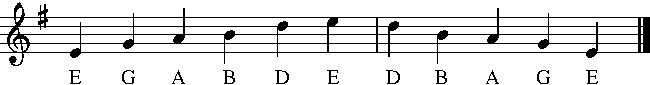
\includegraphics[width=0.95\linewidth]{ly/pentatonic.cropped.pdf}\par
{\small Fingers: E-G-A 1-2-3, thumb under, B-D-E 1-2-3.}
\end{minipage}\hfill
\begin{minipage}[t]{0.47\textwidth}\vspace{0pt}
\sect{Target notes (chord tones)}
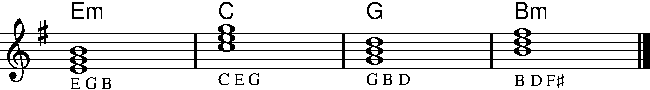
\includegraphics[width=0.95\linewidth]{ly/targets.cropped.pdf}\par
{\small When you lose a note, try these three first.}
\end{minipage}

\sect{Phrase finder}
Play one phrase of the recording, pause, sing its first note, then find it on the keys. Start with the chord tones of the chord underneath. Write what you find.\par\vspace{2pt}
\small
\renewcommand{\arraystretch}{1.55}
\begin{tabularx}{\textwidth}{|l|c|X|X|X|}
\hline
\textbf{Section} & \textbf{Phrase} & \textbf{First note} & \textbf{Longest note} & \textbf{Chord under it}\\\hline
verse & 1 &&&\\\hline
verse & 2 &&&\\\hline
pre-chorus & 1 &&&\\\hline
pre-chorus & 2 &&&\\\hline
chorus & 1 &&&\\\hline
chorus & 2 &&&\\\hline
\end{tabularx}\normalsize

\begin{fivemin}
\tm{0:00--1:00} & \textbf{E minor pentatonic} up and down, right hand, saying the note names.\\
\tm{1:00--2:30} & \textbf{Improvise.} Left hand plays B1 roots round the verse loop; right hand uses only pentatonic notes. End every 4 bars on E, G or B.\\
\tm{2:30--4:00} & \textbf{Phrase finder.} One or two phrases a day, into the table.\\
\tm{4:00--5:00} & \textbf{The melody so far}, from your sheet or tutorial: right hand alone at 80, phrase by phrase.\\
\end{fivemin}

\begin{ladder}
\lv{L1}{E minor pentatonic, one octave, right hand}{70}
\lv{L2}{Two octaves, up and down}{80}
\lv{L3}{Improvise 8 bars over the verse loop, ending on a chord tone}{80}
\lv{L4}{\textbf{Gate.} Phrase finder filled in for verse and chorus}{---}
\lv{L5}{Verse and chorus melody, right hand alone}{80}
\lv{L6}{Melody with left-hand B1 roots}{80}
\lv{L7}{Melody with left-hand B2 or B3}{112}
\end{ladder}

\bottom{Sing the melody while playing the chords from Drill 4. Enter a phrase into a DAW piano roll from memory, then compare it with the record.}
{Singers phrase ahead of and behind the beat. Learn the notes straight, on the grid, first. Copy the looseness from the recording last.}

\newpage
%===================================================== PUT IT TOGETHER
{\fontsize{22}{24}\selectfont\bfseries Put It Together}\par
{\itshape Fill in the map from the recording, then climb the five versions of the song.}\par
\vspace{2pt}\noindent\rule{\textwidth}{0.8pt}

\sect{Song map}
Bar counts come from Drill 1. The recording may have more sections than listed (a second verse, a bridge, an outro); add them in the empty rows. Your notes win over this page wherever they disagree.\par\vspace{3pt}
\small
\renewcommand{\arraystretch}{1.6}
\begin{tabularx}{\textwidth}{|l|l|c|X|X|}
\hline
\textbf{Section} & \textbf{Chords} & \textbf{Bars} & \textbf{Right hand (drill)} & \textbf{Left hand (Drill 5)}\\\hline
Intro & Em C G Bm & & broken chords (8) & B1 roots\\\hline
Verse & Em C G Bm & & 3-3-2 (6) & B2 root--5th\\\hline
Pre-chorus & C G Em D, C G Am D & & 3-3-2 (6) & B2, then B3\\\hline
Chorus & C G Em D \dots & & pushes (7) & B3 8ths or B5 octaves\\\hline
Ending & C D G & & held chords & B1 roots\\\hline
 & & & & \\\hline
 & & & & \\\hline
 & & & & \\\hline
\end{tabularx}\normalsize

\sect{Five versions of the song}
Each version is a complete performance. Play V1 all the way through before you add anything.\par\vspace{3pt}
\begin{ladder}
\lv{V1}{\textbf{Chords.} Lazy shapes, whole notes, left-hand roots, whole form without stopping (Drills 3--4)}{90}
\lv{V2}{\textbf{Groove.} Verse on S4, chorus with pushes and B3 8ths (Drills 5--7)}{112}
\lv{V3}{\textbf{Accompaniment.} V2 with a broken-chord intro; hum or sing the melody over it (Drill 8)}{112}
\lv{V4}{\textbf{Melody.} Melody in the right hand, left hand B1 or B2 (Drill 9)}{80--112}
\lv{V5}{\textbf{Play along} with the recording from start to finish}{record}
\end{ladder}

\sect{Progress log (write the date when you tick a level)}
\small
\renewcommand{\arraystretch}{1.55}
\begin{tabularx}{\textwidth}{|l|*{7}{X|}}
\hline
\textbf{Drill} & \textbf{L1} & \textbf{L2} & \textbf{L3} & \textbf{L4} & \textbf{L5} & \textbf{L6} & \textbf{L7}\\\hline
1 Lock to 112 &&&&&&&\\\hline
2 The Six Chords &&&&&&&\\\hline
3 Lazy Hands: Verse &&&&&&&\\\hline
4 Lazy Hands: Chorus &&&&&&&\\\hline
5 The Left Hand &&&&&&&\\\hline
6 Hands Together &&&&&&&\\\hline
7 The Push &&&&&&&\\\hline
8 Broken Chords &&&&&&&\\\hline
9 Melody by Ear &&&&&&&\\\hline
\end{tabularx}

\end{document}
